\documentclass[12pt, a4paper]{article}
\usepackage[utf8]{inputenc}
%\usepackage[IL2]{fontenc}
\usepackage[czech]{babel}
\usepackage[pdftex]{graphicx}
\usepackage{mathtools}
\usepackage{amsmath}
\usepackage{svg}
\usepackage{textcomp}
\usepackage{listings,xcolor}
\usepackage[final]{pdfpages}
\usepackage{verbatim}
\usepackage{fancyhdr}
\usepackage[T1]{fontenc}
\usepackage{pdfpages}

\usepackage[nottoc,notlot,notlof]{tocbibind}
\usepackage[pdftex,hypertexnames=false]{hyperref}
\hypersetup{colorlinks=true,
  unicode=true,
  linkcolor=black,
  citecolor=black,
  urlcolor=black,
  bookmarksopen=true}

\title{\textbf{Dokumentace semestrální práce} \\KIV/SAR}
\author{Vojtěch Danišík, Jan Čarnogurský}
\begin{document}

\begin{titlepage}
	\newcommand{\HRule}{\rule{\linewidth}{0.5mm}}
	\begin{center}
	
\includegraphics[width=12cm]{img/fav_logo}\\
	\end{center}
	\textsc{\LARGE Západočeská univerzita v Plzni}\\[1.5cm]
	\textsc{\Large Výkonnost a spolehlivost prog. systémů}\\[0.5cm]
	\textsc{\large KIV/VSS}\\[0.5cm]
	\HRule\\[0.4cm]
	{\huge\bfseries Dokumentace semestrální práce}\\[0.4cm]
	\HRule\\[1.5cm]

	\begin{minipage}{0.4\textwidth}
		\begin{flushleft}
			\large
			Vojtěch \textsc{Danišík}\newline
			A19N0028P\newline
			danisik@students.zcu.cz
		\end{flushleft}
		\begin{flushleft}
			\large
			Jan \textsc{Čarnogurský}\newline
			A19N0025P\newline
			cagy@students.zcu.cz
		\end{flushleft}
	\end{minipage}
	\vfill\vfill\vfill
	\vfill
\end{titlepage}
\newpage
\tableofcontents
\newpage

\section{Zadání}
\noindent Zadání semestrální práce spočívalo v implemetaci simulaci vězňovo dilema (Prisonner\textquotesingle s dilemma)

Aplikace bude sestavena ze dvou částí. V první části půjde o to, postavit proti sobě dvě strategie, pro ukázku jejich chování. V této části bude tedy
 možné navolit dvě strategie, které se proti sobě spustí a počet kol (iterací).

Druhá část bude sloužit pro navolení několika strategií proti sobě a nalezení té nejlepší. Bude možné navolit i různé modifikace, které ovlivní chování těchto strategií. Mezi
možné modifikace bude patřit rušení při rozhodnutí, úprava rozhodnutí na základě pamatování minulých her se soupeřem, mutace a rychlost simulace.

\section{Vězňovo dilema}

\noindent Vězňovo dilema (Prisonner\textquotesingle s dilemma) je situace, kdy jsou dva vězni drženi ve dvou oddělených celách. Z toho vyplývá, že nemají možnost mezi sebou komunikovat, a proto nemohou spolu spolupracovat na svých výpovědích. Každý z nich se může řídit jednou z těchto strategií: zapírat nebo se přiznat.

Nastane\-li situace, kdy budou oba zapírat, odsedí si ve vězení kratší dobu, protože na jejich usvědčení ze závažného zločinu nebude mít policie dostatek důkazů a budou usvědčeni pouze ze zločinu méně závažného. Oba dva vězni si v tomto případě odnesou trest kratší ve výši \textit{x} let. Pokud se však jeden z vězňů přizná a zároveň udá druhého vězně, doba pobytu ve vězení se mu (jako odměna za udání spolupachatele) zkrátí a straví ve vězení pouze \textit{y} let. Avšak vězni, který stále zapíral a nepřiznal se, bude doba pobytu ve vězení prodloužena na \textit{z} let, protože již má policie dostatek důkazů pro jeho usvědčení ze závažnějšího trestného činu. Poslední možností je, že se oba dva vězni přiznají. Jakmile nastane tato situace, budou oba dva vězni odsouzeni na \textit{w} let.

Tato situace nám uakzuje dilema, které vzniká mezi vězni proto, že se nemohou mezi sebou domluvit na již zmíněných strategiích. Pro každého z nich je nejlepší se přiznat a zároveň udat toho druhého. Jenomže žádný z vězňů neví, jak bude reagovat druhý vězeň. Kdyby se mohli domluvit, tak nejlepšími strategiemi by pro oba vězně bylo zapírat, přičemž by oba ve vězení strávili \textit{x} let.

\section{Řešení}
\noindent Semestrální práci jsme se rozhodli řešit v technologiích HTML, CSS a JS. Důvodem pro zvolení těchto technologií byla jenoduchost nasazení na webový server bez nutnosti
serverové části pro logiku aplikace.

\nointent Semestrální práce se skládá ze tří webových stránek:

\subsection{Strategie}
\noindent V semestrální práci byly implementovány následující strategie. Spoluprací se myslí spolupráce s policií.
\begin{itemize}
  \item ALLC - Vždy spolupracuje
  \item ALLD - Vždy zradí
  \item ALT - Začne spoluprací, pak střídá spolupráci a zradu
  \item APP - Začne spoluprací, pokud protivník spolupracoval opakuje předchozí tah, jinak provede opačný tah
  \item CPAVG - Rozhodnutí na základě předchozích protivníkovo tazích. Pokud protivník ve 20\% spolupracoval, je 20\% šance, že bude spolupracovat i on s ním.
  \item GRIM - Spolupracuje dokud ho nezradí, potom neustále zrazuje.
  \item PAV - Začne spoluprací, následně opakuje předchozí tah pokud měl pozitivní výsledek, jinak udělá opak.
  \item RAND - Náhodný tah.
  \item TFT - Začne spolupracovat, pak kopíruje tahy protivníka.
  \item TFTT - Vždycky spolupracuje, dokud protihráč dvakrát nezradí.
  \item TTFT - Vždycky spolupracuje, dokud protihráč nezradí alespoň jednou v posledních dvou tazích.
\end{itemize}

\newpage
\subsection{Domovská stránka}
\noindent Obsahuje základní popis vězňovo dilema a popis implementovaných strategiích.

\subsection{Základní porovnání dvou strategií}
\noindent Obashuje výběr dvou strategií ze seznamu, s možnostní navolení počtu her. Simulace se spouští stisknutím tlačítka \uv{Visualize}, které je zneaktivněno do dokončení simulace. Výsledky jsou následně vkládány do tabulky pod tlačítkem.


\noindent V tabulce jsou na řádcích zobrazeny jednotlivé výsledky her. Jednotlivé hodnoty v sloupci u vězně dopovídají:
\begin{itemize}
  \item celkové skóre
  \item ikona - spolupráce s policií (zelená ikona s palce), nespolupráce s policií (červená ikona se zkříženými prsty)
  \item + body - počet bodů získaných v daném kole
\end{itemize}

Pod tabulkou je vypočítané celkové skóre vězně. Vyhrává ten vězeň, který má méně bodů. Logika bodů odpovídá k počtu roků za mřížemi.


\begin{figure}[!h]
  \centering
  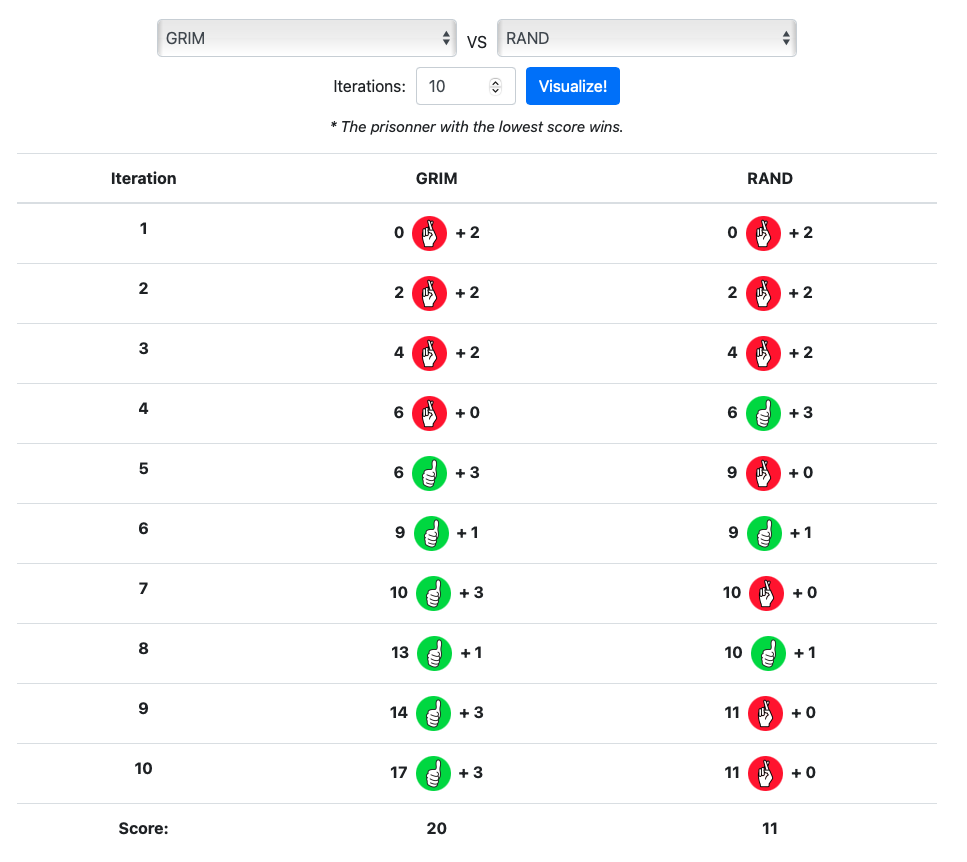
\includegraphics[scale=0.25]{img/basic.png}
  \caption{Ukázka porovnání strategií}
\end{figure}
\newpage


\subsection{Porovnání více strategií}
\noindent Na této stránce je možné navolit několik strategií a porovnat je mezi sebou. Strategie se přidávají pomocí tlačítka \uv{+} a simulace se spouští tlačítkem \uv{Visualize}. Během simulace je tlačítko zneaktivněno.

U každé simulace je možná nadefinovat několik možností, které mohou simulaci ovlivnit. Detailní popis implementace modifikátorů je popsán v následující kapitole.

\begin{itemize}
  \item iterace - Počet kol
  \item rušení - Možnost zapojení rušení do algoritmu strategie. Hodnoty 0 - 100\%
  \item mutace - Po každé iteraci se nejsilnější stragerie rozmnoží a nahradí nejslabšího. Simulace běží dokud výsledek nekonverguje k nějaké strategii.
  \item pamatování historie - Ovlivnění rozhodnutí s přihlednutím k minulým hrám.
  \item rychlost - Ovlivnění rychlosti simulace.
\end{itemize}

Výsledky jsou reprezentovány pomocí dvou grafů. První graf slouží pro zobrazování skóre jednotlivých vězňů/strategií. V druhém grafu je znázorněno zastoupení strategií v populaci.

\begin{figure}[!h]
  \centering
  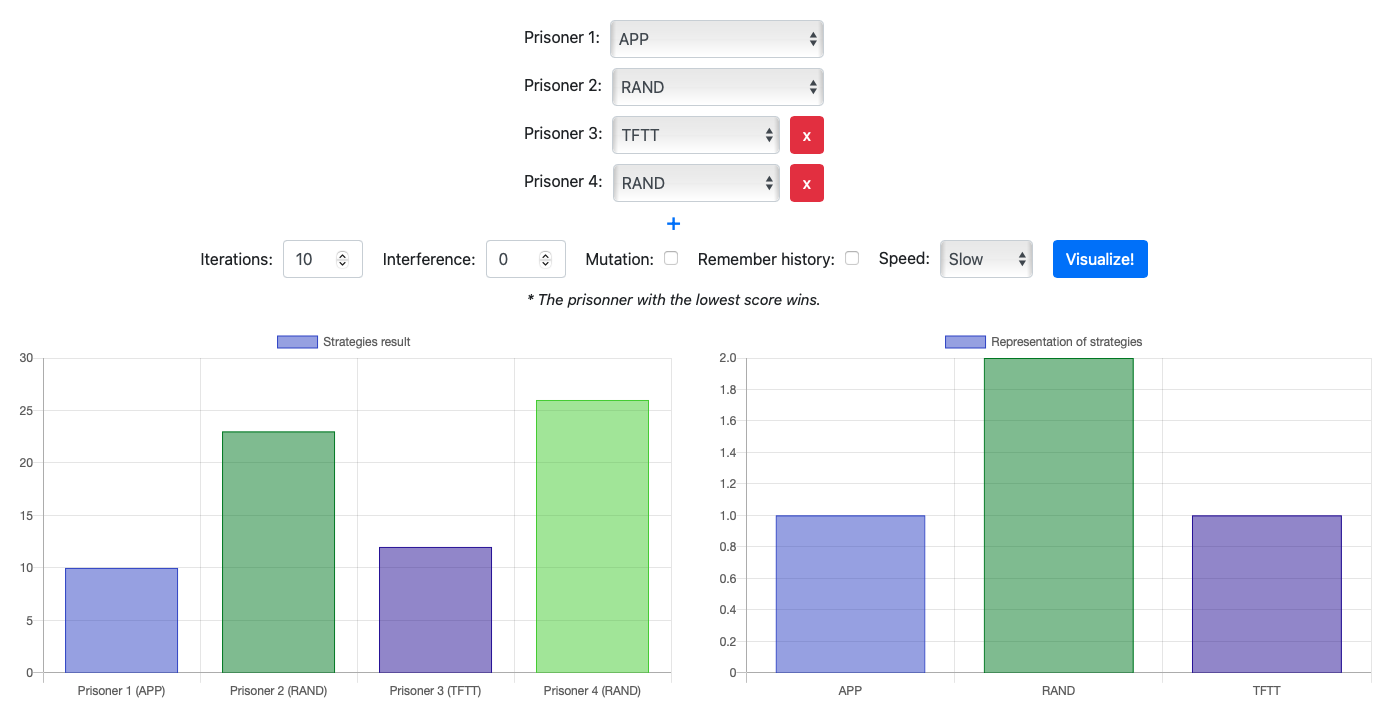
\includegraphics[scale=0.3]{img/iter.png}
  \caption{Ukázka porovnání více strategií}
\end{figure}
\newpage

\section{Implementace}
\subsection{Jednotlivé strategie}
\noindent Popis algoritmů jednotlivých strategií je umístěn v souboru \textit{js/algorithms.js}.

\subsection{Porovnání více algoritmů - výběr protivníků}
Vojta

\subsection{Rušení}
Vojta


\subsection{Mutace}
Vojta


\subsection{Pamatování minulých her}
Vojta

\subsection{Grafy}
\noindent Pro zobrazení výsledků v grafech, byla použita knihovna Chart.js. Knihovna umožnuje celkem snadno nadefinovat nastavení grafu i s jeho hodnotami, které je možné dynamicky měnit.

Grafy jsou inicializovány metodou \textit{initGraphs()}. U grafů jsou inicializovány osy, nastavení barev a název grafu.

Hodnoty grafu se skórem jsou nastavovány metodou \textit{updatePoints()}, která je volána po každé iteraci. V cyklu se projdou všichni vězni a získají se jejich body, které jsou následně namapovány pro graf. Tato data se nastaví do grafu a provede se update grafu.

Hodnoty zastoupení strategií jsou nastavovány metodou \textit{updateRepresentation()}. Metoda je volána ihned po inicialitaci grafů a při simulaci se mění pouze při provedení mutace. V cyklu se projdou vězni a zjistí se zastoupení četnosti strategií. Tato data jsou následně namapována a poslána do grafu.

\section{Struktura souborů}
\nointent Adresářová struktura s popisem jendotlivých souborů. Jsou vynechány soubory, které jsou součástí externích knihoven (Bootstrap, jQuery, Chart).

\begin{itemize}
  \item \textit{index.html} - Domovská stránka webu
  \item \textit{basic.html} - Stránka s porovnáním dvou algoritmů
  \item \textit{iteration.html} - Stránka s porovnáním více strategií
  \item \textit{css/style.css} - Popis kaskádových stylů
  \item \textit{js/algorithms.js} - Implementace rozhodnutí jednotlivých strategií
  \item \textit{js/classes.js} - Popis jednotlivých tříd
  \item \textit{js/utils.js} - Obecné funkce použité napříč stránkami
  \item \textit{js/basic.js} - Obsluha výpočtu i porovnání dvou algoritmů
  \item \textit{js/iteraction.js} - Obsluha interakce s uživatelem na stránce s porovnáním více algoritmů
  \item \textit{js/iteration.js} - Obsluha výpočtů na stránce s porovnáním více algoritmů
\end{itemize}

\section{Licence}
\noindent Níže je seznam použitých knihoven s jejich licence:
\begin{itemize}
  \item Bootstrap - MIT
  \item jQuery - MIT
  \item Chart.js - MIT
\end{itemize}



\section{Závěr}
V semestrální práci jsme implementovali simulaci na téma vězňovo dilema. V první části je možné porovnat dvě strategie proti sobě a v druhé simulovat více strategií proti sobě s různými modifikacemi. 

Od začátku jsme semestrální práci dělali tak, aby napodobovala použitelnost simulace markovských modelů, která byla zpracována jako semestrální práce v minulých letech. Šlo nám o to, vytvořit \uv{něco}, co by mohlo sloužit jako výukový materiál v budoucích letech.


\end{document}
